\chapter{Planar Separator Theorem}

\section{Planar Separator Algorithm}
\begin{defn}
    A set $S \subseteq V(G)$ is a separator if induced graph $G^* = G - S$
    has at least two connected components $A,B \subseteq G^*$.
\end{defn}

Through the years, more and more classes of graphs started to show some
interesting properties regarding vertex separators, so a general theorem was
assembled, which is called a $f(n)$-separator theorem:
\begin{theorem} \cite{liptonSeparatorTheoremPlanar1979} \label{thm:fnseparator}
    Let $S$ be a class of graphs closed under a subgraph relation (i.e. if
    $G_1 \in S$ and $G_2$ is a subgraph of $G_1$, then $G_2 \in S$). There
    exist constants $\alpha < 1$, $\beta > 0$ such that if $G$ is any n-vertex
    graph in $S$, the vertices of $G$ can be partitioned into three sets $A,B,C$
    such that no edge connects any vertex in $A$ and $B$, neither $A$ nor $B$
    have more than $\alpha n$ vertices and $C$ contains no more than $\beta
    f(n)$ vertices
\end{theorem}

Such theorem regarding planar graphs, where $f(n) = O(\sqrt{n}),$ $ \alpha = 2/3,
$ $\beta = 1$ is called planar separator theorem. First breakthrough in that area
was in 1951 \cite{ungar1951theorem}, when Ungar proved a slightly weaker theorem
with $f(n) = O(\sqrt{n} \log^{3/2}n)$. A small improvement to that was later
achieved in 1973 by George \cite{george1973nested} where he proved that any
grid graph of size $n$ has a $O({\sqrt{n}})$ separator. However, the first to
prove planar separator theorem in the full form were Lipton and Tarjan in 1977
\cite{liptonSeparatorTheoremPlanar1979}, where it was proven that for each
planar graph a separator of size at most $2\sqrt{2} \sqrt{n}$ exists.
In many articles later after Lipton and Tarjan, the constant $\beta$ was
reduced, however its lower bound is $(\sqrt{4\pi \sqrt{3}})/3$ which was proven
by Djidjev in \cite{djidjev1982problem}.
Djidjev established this absolute limit not by looking at flat grids,
but by constructing worst-case planar graphs based on the triangulation
of a sphere, proving mathematically that no algorithm can separate
these dense spherical meshes with fewer vertices.

The main theorem, this whole thesis and all algorithms are based
on is the planar separator theorem introduced by Lipton and Tarjan.
However at first we shall define rigorously what a separator is.

What is really interesting about this theorem is that it holds even if we 
assign some cost to any vertex, and partition the graph based on that.
However, at first we shall make a formal definition for that generalization.

\begin{defn} \label{defn:weighted}
    Vertex-weighted graph $G$ is a tuple $(V, E, w)$, where $V$ is called
    a vertex set, $E$ are 2-element subsets of $V$ and $w \colon V \rightarrow \mathbb{R}^+ \cup \{0\}$
    is a weight function. In the remainder of this paper we shall refer to weight of a vertex
    as \textit{cost} of a vertex. Moreover we will refer to vertex-weighted graphs 
    as \textit{weighted graphs}.
\end{defn}

We can extend the definition of a weight function for a single vertex to a weight 
function for a whole graph.

\begin{defn} \label{defn:cost-fun}
    Let $G = (V, E, w)$ be a weighted graph. Let $W \colon G \rightarrow \mathbb{R}^+ \cup \{0\}$
    be defined as $W(G) = \sum_{v \in V} w(v)$. We shall call $W(G)$ the cost of a graph $G$.
    Moreover, let $X \subseteq V$, we will define $W(X)$ as the cost of a set of vertices $X$.
\end{defn}

\needspace{6\baselineskip}

\begin{theorem}[Planar Separator Theorem \cite{liptonSeparatorTheoremPlanar1979}]\label{thm:planar-separator}
	Let $G = (V, E, w)$ be a weighted planar graph with $n$ vertices, such that
    $W(G) \leq 1$. Then we can partition
	vertices of $G$ into three sets $A$, $B$, and $C$ such that:
    \begin{enumerate}
        \item[(a)] there exists no edge ${u, v} \in E$ with $u \in A$ and $v \in B$,
        \item[(b)] $W(A) \leq 2/3$ and $W(B) \leq 2/3$,
        \item[(c)] $|C| \leq 2\sqrt{2}\sqrt{n}$. 
    \end{enumerate}
	
    \noindent
	Moreover, such a partition can be found in $O(n)$ time.
\end{theorem}

To prove this theorem we will base on a few already proven facts on planar
graphs as well as some lemmas, that we will introduce ourselves.

\subsection{BFS layering} \label{section:bfs}
One of the most important parts of the proof of
Theorem~\ref{thm:planar-separator} is the concepts of layers which are levels of
a BFS spanning tree.
\begin{defn}
    Let $G = (V, E)$ be a connected planar graph and $t \in V$ be a vertex that we
    will call the root of a tree. A BFS spanning tree is a tree $T$ rooted in
    $t$ such that $\forall_{v \in V(G)} \, d_T(t, v) = d_G(t, v)$.
\end{defn}

Using this spanning tree we can partition the vertex set $V$ into disjoint sets
that we will call layers (or levels). So we can define it as $L_i = \{ u
\in V \colon d(t, u) = i\}$ (clearly, $L_0 = \{ t \} $).
Such a layering has two important properties that will be very useful in the
future.
\begin{lemma}\label{lem:neighborhood}
    If $(u, v) \in E$ and $u \in L_i, v \in L_j$, then $|i - j| \leq 1$.
\end{lemma}
The proof for this lemma is very simple by following the construction of BFS
spanning tree during BFS traversal. The other property is also very intuitive
and follows directly from Lemma~\ref{lem:neighborhood}.
\begin{lemma} \label{lem:separation}
    For any $l \in \{ 1, \dots, r-1 \}$ removal of $L_l$ from $G$ separates it into two disconnected components
    $\bigcup_{i=0}^{l-1} L_i$ and $\bigcup_{i=l+1}^{r} L_i$
\end{lemma}

It is easy to see that this lemma shows connection between BFS layering and 
separation of components, and we shall see how it is incorporated into the proof
for the main theorem in near future. Another separating property can be derived
for planar graphs specifically.

\begin{theorem} \cite{liptonSeparatorTheoremPlanar1979} \label{thm:jordan-curve}
    Let $C$ be any closed curve in the plane. Removal of $C$ divides the plane
    into exactly two connected regions: "inside" and "outside" of $C$.
\end{theorem}

Although the proof for this theorem is pretty formal and uses topological properties
of the plane, intuition for it is pretty straightforward. As the edges in a planar 
graphs cannot cross on the plane, a closed curve is a natural separator, as no edge
from a vertex on \textit{outside} can cross the curve to reach any vertex on \textit{inside}.

\subsection{Fundamental cycle}
The first lemma needed to prove Theorem~\ref{thm:planar-separator} shows us how 
the intuitive separation property from Theorem~\ref{thm:jordan-curve} can be used
to get the needed costs of separated subgraphs. To do this we will need the concept 
of a fundamental cycle.
\begin{defn}\label{def:fundamental_cycle}
Let $G = (V, E)$ be a graph and let $T$ be a spanning tree of $G$.
For any non-tree edge $e = (u, v) \in E \setminus E(T)$, the unique simple cycle
consisting of $e$ and the unique path in $T$ connecting $u$ and $v$
is called the \emph{fundamental cycle} defined by $e$.
\end{defn}
As we can see from this definition, fundamental cycles can be defined if we have 
a spanning tree for a graph. It connects with BFS layering defined earlier, and in 
the next section we will explore this further. However, we begin with the lemma related
to fundamental cycles.
\begin{lemma} \cite{liptonSeparatorTheoremPlanar1979} \label{lem:fundamental_cycle}
    Let $G = (V, E, w)$ be a weighted planar graph with $n$ vertices, such that $W(G) \leq 1$
    . Suppose that $G$ has a spanning tree $T$ with
    radius $r$. Vertices of $G$ can be partitioned into three
    sets $A, B, C$ such that: 
    \begin{enumerate}
        \item[(a)] there exists no edge ${u, v} \in E$ with $u \in A$ and $v \in B$,
        \item[(b)] $W(A) \leq 2/3$ and $W(B) \leq 2/3$,
        \item[(c)] $|C| \leq 2r + 1$ and $C$ contains root of $T$. 
    \end{enumerate}
\end{lemma}
\begin{proof}
    We shall see that if $G$ has a vertex $v$ with cost at least $1/3$, the lemma is
    true. To prove that, let us consider $C = (V_C, E_C)$ to be the path from $v$ to the root of $T$.
    We can see that it
    has less than $2r + 1$ vertices and contains the root. Moreover: $W(V_C) \geq 1/3$
    so if we assign the rest of vertices of $G$ to $A$ and let $B
    = \emptyset$ then the proof is completed. 

    Thus let's assume that $G$ does not have a vertex with cost at least $1/3$.
    Let's now embed $G$ in plane using any algorithm \footnote{As discussed in section below
    \Cref{defn:embedding}},
    and make that graph maximal planar by 
    adding edges, so that each face is a triangle.

    Now each
    one of the non-tree edges (those added when making $G$ maximal as well)
    creates a cycle $C$ with tree edges, its length being at most $2r + 1$.
    From \Cref{thm:jordan-curve}
    we know that $C$ splits the plane into two parts: the \textit{inside} and
    \textit{outside}. If we can prove that there exists a cycle $C$ such that
    neither side contains vertices whose total cost exceeds $2/3$, then the
    lemma is proven.

    Let $(x, z)$ be a non-tree edge that minimizes the maximum cost of either sides of
    the cycle $C'$ that it closes. If there are many edges with this property, pick
    the one with the smallest number of faces on the maximized side. Let's say
    without loss of generality, that the \textit{inside} has the cost at least
    as high as the \textit{outside}. If that cost does not exceed $2/3$ then the
    lemma is true. Otherwise let's consider a triangle $F_T$ inside $C'$ such that
    $(x, z)$ is one of its boundaries. Let $y$ be the third vertex of $F_T$.
    Now we have to do case analysis based on properties of the edges of $F_T$:
    \begin{itemize}
        \item if both $(x, y), (y, z)$ lie on the cycle then $F_T = C'$ , which
        contradicts with the fact that inside has a positive cost, so it has to
        have vertices
    \item if one of $(x, y), (y, z)$ (assume without loss of generality it is
        $(x, y)$) lies on the cycle, then $(y, z)$ is a non-tree edge (it has 
        to be a non-tree edge, as otherwise it would close a smaller cycle $(x, y, z)$,
        which 
        is not possible as $(x, z)$ defines $C'$) that
        defines a new cycle $C''$ with the same cost, but one less face that
        $C'$ which contradicts with choice of $(x, z)$.
        \begin{figure}[H]
            \centering

            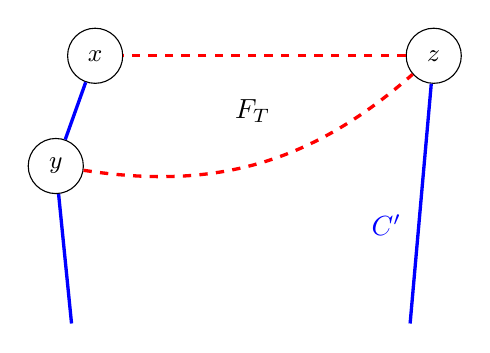
\begin{tikzpicture}[
                vertex/.style={
                    circle,
                    draw,
                    fill=white,
                    minimum size=7mm,
                    inner sep=0pt,
                    font=\small
                },
                tree/.style={
                    very thick
                },
                cycle/.style={
                    very thick,
                    blue
                },
                non-tree/.style={
                    very thick,
                    dashed,
                    red
                },
                ghost/.style={
                    thick
                }
            ]

                \node[vertex] (x) at (0.5,3.4) {$x$};
                \node[vertex] (y) at (0,2.0) {$y$};
                \node[vertex] (z) at (4.8,3.4) {$z$};

                \node[coordinate] (a) at (0.2,0) {};
                \node[coordinate] (b) at (4.5,0) {};

                \draw[cycle] (b) -- (z);
                \draw[cycle] (a) -- (y);

                \draw[cycle] (x) -- (y);
                \draw[non-tree] (z) -- (x);

                \draw[non-tree] (y) to[bend right=25] (z);

                \node[blue] at (4.2,1.25) {$C'$};
                \node[black] at (2.5,2.7) {$F_T$};

            \end{tikzpicture}

            \caption{See how, $(y, z)$ defines a new cycle with one fewer face than $C'$.}
            \label{fig:case2}
        \end{figure}
    \item if none of $(x, y), (y, z)$, we have to make another case analysis
        looking at all possible configurations of those two edges being a tree
        edge. All those configurations lead to a contradiction (a complete proof
        is to be found in \cite{liptonSeparatorTheoremPlanar1979}).
    \end{itemize}
    As we can see, all of the cases lead to contradiction, so the cost inside
    $C'$ has to be at most $2/3$.
\end{proof}

\subsection{Layering}
As forecasted earlier, in this section we will show how we can utilize facts introduced
in \Cref{section:bfs} and just proved \Cref{lem:fundamental_cycle} to show the 
construction of spanning tree $T$ and graph partition. 
\begin{lemma} \cite{liptonSeparatorTheoremPlanar1979} \label{lem:layering}
    Let $G = (V, E, w)$ be a planar graph with $n$ vertices, such that $W(G) \leq 1$
    . Suppose that vertices are partitioned into
    layers using a BFS spanning tree $T$ rooted in $t$ and with radius $r$. Let
    $r+1$ be an additional level with no vertices. Given any two levels $l_1,
    l_2$ such that $\bigcup_{i=0}^{l_1-1} w(L_i) \leq 2/3$
    and $\bigcup_{i = l_2 + 1}^{r+1} w(L_i) \leq 2/3$, it is possible to find a partition of $G$ into
    sets $A, B, C$ such that:

    \begin{enumerate}
        \item[(a)] there exists no edge ${u, v} \in E$ with $u \in A$ and $v \in B$,
        \item[(b)] $W(A) \leq 2/3$ and $W(B) \leq 2/3$,
        \item[(c)] $|C| \leq |L_{l_1}| + |L_{l_2}| + \max \{ 0, 2(l_2 - l_1 - 1) \}$. 
    \end{enumerate}
\end{lemma}

\begin{proof}
    Let's assume that $l_1 \geq l_2$. Then we can select $A =
    \bigcup_{i=0}^{l_1-1} L_i$, $B = \bigcup_{i=l_1+1}^{r+1} L_i$ and $C =
    L_{l_1}$. We can see that the lemma is true, as by definition $W(A) \leq 2/3$  
    and $|C| = |L_{l_1}| \leq |L_{l_1}| + |L_{l_2}| + \max \{ 0, 2(l_2 - l_1 - 1) \}$.
    Moreover, because $l_1 \geq l_2$, then $B \subseteq
    \bigcup_{i=l_2+1}^{r+1} L_i$, so $W(B) \leq \bigcup_{i = l_2 + 1}^{r+1} w(L_i) \leq 2/3$.
    
    Thus suppose $l_1 < l_2$.
    Let's define sets: $D_1 =
    \bigcup_{i=0}^{l_1-1} L_i$, $D_2 = \bigcup_{i=l_1 + 1}^{l_2-1} L_i$, $D_3 =
    \bigcup_{i=l_2 + 1}^{r+1} L_i$, all of which may be empty. We can see that
    they are disjoint by Lemma~\ref{lem:separation}. The only set that
    can have cost exceeding $2/3$ is $D_2$ (by assumptions of this lemma). If
    $W(D_2) \leq 2/3$, then the lemma is true, as we can set
    the most costly part to be $A$, $B$ will consist of the other two parts
    and $C = L_{l_1} \cup L_{l_2}$.
    
    Let's then suppose that the cost of $D_2$ is greater that $2/3$. Delete
    all vertices on levels $l_2$ and above, and shrink levels $0, \dots,
    l_1$ into one vertex $t'$ with cost 0. From Lemma~\ref{lem:shrinking} we know that shrinking
    vertices preserves planarity. We can now see that the new graph $H$ has a
    spanning tree rooted in $t'$ and radius $l_2 - l_1 - 1$.

    Apply Lemma~\ref{lem:fundamental_cycle} to $H$ and let $A_H, B_H, C_H$ be the resulting
    partition. Let $A$ be the set among $A_H$ and $B_H$ that has greater cost
    and let $C$ consist of all of the vertices in $L_{l_1}$, $L_{l_2}$ in the
    original graph G as well as all of the vertices from $C_H - \{ t' \}$. And finally
    $B$ will consist of all of the vertices from $V$ that are not in $A$ or $C$. We
    can see that it works because by Lemma~\ref{lem:fundamental_cycle}, the cost
    of $A$ does not exceed $2/3$. Moreover because of our construction, $C$ has
    the size of at most $|L_{l_1}| + |L_{l_2}| + 2(l_2 - l_1 - 1)$. However we can see
    that the cost of $A \cup C_H$ has to be at least $1/3$, as $A$ was the set
    with greater cost among $A_H, B_H$, hence $W(B) \leq 2/3$.
\end{proof}

\subsection{Main theorem}
Now we have all of the tools to tackle Theorem~\ref{thm:planar-separator}.
\begin{proof}
Assume at first that $G$ is connected. At first we partition into layers using
BFS layering getting a spanning tree $T$ rooted in $t$ with radius $r$.
Additionally we define two empty boundary levels $L_{-1}$ and $L_{r+1}$. Let us
define $l_1$ as the number of the level such that the cost of vertices included in
levels $0$ through $l_1 - 1$ is strictly less than $1/2$ and the cost of
vertices in levels $0$ through $l_1$ be at least $1/2$.

If no such level exists
then the cost of vertices is less or equal than $1/2$, and such we can assign $A = V$,
$B = C = \emptyset$, thus the theorem is true.

We shall define $k = \sum_{i=0}^{l_1}L(i)$. Now, we find two levels:
\begin{itemize}
    \item $l_0$ such that $l_0 \leq l_1$ and $|L_{l_0}| + 2(l_1 - l_0) \leq 2
        \sqrt{k}$
    \item $l_2$ such that $l_1 + 1 \leq l_2$ and $|L_{l_2}| + 2(l_2-l_1-1) \leq 2
        \sqrt{n - k}$
\end{itemize}
If $l_0, l_2$ exist then by Lemma~\ref{lem:layering} (as by definition of
$l_1$ and thus $l_0, l_2$ conditions for it hold) we have a partition $A, B, C$
and the cost of $C$ does not exceed $2(\sqrt{k} + \sqrt{n-k})$.

Now by employing
Cauchy-Schwartz inequality:
$$
    (u_1v_1 + u_2v_2)^2 \leq (u_1^2 + u_2^2)(v_1^2 + v_2^2)
$$
with $u^T = [2, 2]$ and $v^T = [\sqrt{k}, \sqrt{n - k}]$ we can deduce that the
cost of $C$ is bounded by $2\sqrt{2} \sqrt{n}$.
Now we shall see that such levels $l_0$ and $l_2$ exist. Let's suppose that
$l_0$ does not exist. Then for $\forall_{i \leq l_1} |L_{i}| \geq 2 \sqrt{k} -
2(l_1 - i)$. As $|L_0| = 1$ we have $1 \geq 2\sqrt{k} - 2l_1$ and thus
$l_1 + 1/2 \geq \sqrt{k}$. If we take the floor of that we have that $l_1 \geq
\left \lfloor{\sqrt{k}}\right \rfloor$. And now by definition of $k$ we have:
\begin{align*}
    k &= \sum_{i=0}^{l_1} L(i) \overset{(1)}{\geq} \sum_{i=l_1 - \sqrt{\left
\lfloor{k}\right \rfloor}}^{l_1} L(i)
\overset{(2)}{\geq} \sum_{i=l_1 - \sqrt{\left \lfloor{k}\right \rfloor}}^{l_1} 2\sqrt{k} - 2(l_1 - i) \\
      & \overset{(3)}{\geq} (4\sqrt{k} - 2 \sqrt{\left \lfloor{k}\right
          \rfloor}) (\sqrt{\left \lfloor{k}\right \rfloor} + 1)/2
          \geq \sqrt{\left \lfloor{k}\right \rfloor}(\sqrt{\left
      \lfloor{k}\right \rfloor} + 1) > k
\end{align*}
Inequality $(1)$ comes from the fact that we can restrict the range over which
we sum as $l_1 + 1/2 \geq \sqrt{k}$. Inequality $(2)$ stems from the fact that
$L(i) \geq 2 \sqrt{k} - 2(l_1 - i)$. And inequality $(3)$ comes from the
arithmetic sum formula. And thus we can see a contradiction, so $l_0$ exists.
An analogous, symmetric proof can be given for $l_2$ existence. This concludes
proof for a connected graph. \\
If $G$ is not connected, let $G_1, \dots, G_k$ be connected components of $G$.
If no connected component has cost exceeding $1/3$, then let $i$ be the minimum
index such that the cost of $V(G_1), \dots, V(G_i)$ exceeds $1/3$. Then we
can set $A = V(G_1) \cup \dots V(G_i)$, $B = V(G_{i+1}) \cup \dots V(G_k)$ and
$C = \emptyset$ and find our partition. When there is some component with cost
at least $1/3$ and not exceeding $2/3$ let's say $G_j$, then we can set $A =
V(G_j)$, $B = V(G) \setminus V(G_j)$, $C = \emptyset$ and find our partition.
If there is some component with cost at least $2/3$ then we can employ for that
connected component an argument in the first section of this proof to find a
partition $A^*, B^*, C^*$. We can then set $C = C^*$, $A$ will be the vertex set
among $A^*$ and $B^*$ that has the greater cost and $B$ shall be the rest of the
vertices in the graph. It is easy to see that this concludes our proof.
\end{proof}
\subsubsection{$O(n)$ Algorithm}
Following the constructions used in order to proof
Theorem~\ref{thm:planar-separator}, Lipton and Tarjan developed an $O(n)$
algorithm to find a partition described in it. On the input we get a planar
graph $G$ for example in adjacency lists representation
\begin{enumerate}
    \item Find a planar embedding of $G$ using an efficient $O(n)$ algorithm
        \footnote{As discussed in section below \Cref{defn:embedding}}.
    \item Find connected components of $G$ and calculate costs of each one. If
        there is no connected component with cost at least $2/3$, then follow the last part of
        the proof for Theorem~\ref{thm:planar-separator}. Otherwise, go to the
        next step.
    \item Find a BFS spanning tree of the most costly component. Compute the
        level of a vertex and for each level compute $|L_l|$.

    \item Find $l_1$ such that the cost of levels $0, \cdots, l_1 - 1$ does not
        exceed $1/2$ and the cost of levels $0, \cdots, l_1$ is greater or equal
        that $1/2$. Now find the highest level $l_0 \leq l_1$ such that
        $L(l_0) + 2(l_1 - l_0) \leq 2 \sqrt{k}$ and lowest level $l_2 \geq l_1 +
        1$ such that $L(l_2) + 2(l_2-l_1-1) \leq 2 \sqrt{n - k}$.

    \item Delete all vertices on level $l_2$ and above. Construct a new vertex
        $x$ and shrink all the levels from 0 to $l_0$ to that one vertex,
        rewiring the edges on the boundary of $l_0$ level to $x$ 
        \footnote{See \cite{liptonSeparatorTheoremPlanar1979} or \texttt{LiptonTarjanPlanarSeparator.cpp}
        from Chapter 4}. 

    \item Construct a BFS spanning tree $T_x$ rooted in $x$. Keep track for each
        vertex $v$ of its parent in $T_x$ and the total cost of descendants of
        $v$ including $v$ itself. Make the graph maximal by triangulation.

    \item Choose any non-tree edge $(v_1, w_1)$ and by following parent pointers
        find a corresponding fundamental cycle $C_1$. Compute costs of either sides of the
        cycle.

    \item By Theorem~\ref{thm:jordan-curve} we know that a cycle 
        splits the plane into two sides: inside and outside. Let's call the set of 
        vertices on the inside $X_I$ and the set of vertices outside $X_O$. Using
        Algorithm~\ref{alg:fundamental_cycle} (with input being $C_1$ found in the previous step)
        find a fundamental cycle $C$ such 
        that $W(X_I) \leq 2/3$ and $W(X_O) \leq 2/3$ .

    \item Use the cycle found in the previous step and levels found in step 4
        to construct a vertex partition as described in proof for
        Lemma~\ref{lem:layering}. Extend the partition found for the most costly
        connected component to entire graph like in the proof for
        Theorem~\ref{thm:planar-separator}.
\end{enumerate}
\subsubsection*{Time complexity}
It is easy to see that all the steps, but steps 7 and 8, take $O(n)$ time.
So let's prove that for both of them as well.
\begin{lemma}
    Step 7 of Lipton-Tarjan Planar Separator Algorithm takes $O(n)$ time.
\end{lemma}
\begin{proof}
    At first we shall define what is the lowest common ancestor, which in our case
    will be a vertex reached by following parent pointers from $v_1$ and $w_1$.
    \begin{defn}
        Let $T = (G, V)$ be a tree rooted in $t$. For $v, w \in T$ consider paths 
        $P_v = (V_1, E_1)$ and $P_w = (V_2, E_2)$ such that $V_1 = \{v, \cdots, t\}$
        and $V_2 = \{w, \cdots, t\}$. The lowest common ancestor (\emph{LCA} in short) 
        of $v$ and $w$ is a vertex $x$, such that $x \in V_1 \cap V_2$ and $d(x, t)$ is 
        the largest among all of the vertices in $V_1 \cap V_2$ ($x$ is the deepest in $T$
        among them).
    \end{defn}
    In step 7 we find the cycle $C_1$ by finding \emph{LCA} of $v_1$ and $w_1$ which can
    easily be done in $O(n)$ time by following parent pointers computed in Step 6. 
    The cycle consists of paths from $v_1$ and $w_1$ to their \emph{LCA} and a non-tree 
    edge $(v_1, w_1)$.
    To compute the costs of both sides, for each vertex in the cycle
    we can look at the embedding. Let's consider vertex $v \in C_1$. The planar embedding 
    gives us a cyclic order on its incident edges. Each one of these edges is on the inside 
    of the cycle, outside of the cycle or on the cycle (by \Cref{thm:jordan-curve}). 
    Now we can use precomputed costs of vertices and their subtrees from Step 6 to find 
    the contribution of a subtree hanging of each one of these edges to their respectable side 
    in $O(1)$ time. And as the number of scanned edges is $O(n)$, then the whole step is linear.
\end{proof}
 
Now we can move on to prove that Step 8, which is described in \Cref{alg:fundamental_cycle} is linear.
\begin{lemma}\label{lem:fundamental_cycle_algo}
    Algorithm~\ref{alg:fundamental_cycle} has time complexity $O(n)$.
\end{lemma}
\begin{proof}
    In each step of the algorithm we remove at least one face of the planar
    graph, so the number of iterations is bound by $O(n)$.

    In each iteration we
    do some $O(1)$ work, work proportional to the length of path $P_T$ and some
    work proportional to the number of edges scanned in cycles $R_1, R_2$. We
    can see that if $e \in P_T$, then that computation regarding tree path is
    done only once, as that edge will in the next iteration be on the boundary
    of new cycle.

    So all the work regarding computations of $P_T$ amortizes to
    $O(n)$. Regarding scanning, we can see that if we scanned $k$ edges in each
    cycle before stopping we did computations proportional to $O(k)$. But in the
    next iteration at least $k$ edges will be outside the next cycles. So those
    computations amortize to $O(n)$ as well.
\end{proof}
        \begin{algorithm}[H]
            \small
    \caption{$\text{FUNDAMENTAL\_CYCLE}$}
    \label{alg:fundamental_cycle}
    \begin{algorithmic}[1]
        \Require $C_1$
        \State $i \gets 1$
        \State $C_i \gets C_1$
        \State Let $(v_i, w_i)$ be a non-tree edge completing $C_i$
        \While{cost inside $C_i$ exceeds $2/3$}
        \State Let $(v_i, y, w_i)$ be a triangle inside $C_i$ with boundary edge
        $(v_i, w_i)$
        \If{$(v_i, y) \in E(T_x)$ $\mathbf{or}$ $(w_i, y) \in E(T_x)$}
        \State Let $(v_{i+1}, w_{i+1})$ be a non-tree edge among $(v_i, y),
        (w_i, y)$
        \State Let $C_{i+1}$ be a cycle defined by $(v_{i+1}, w_{i+1})$
        \State Compute cost inside $C_{i+1}$
        \Else
        \State Find tree path $P_T$ from $y$ to $C_i$ path
        \State Let $z$ be the first vertex in $P_T$ from $y$ that is on $C_i$
        \State Compute cost of all vertices on $P_T \setminus \{z\}$
        \State We have two cycles $R_1$ defined by $(y, v_i)$ and $R_2$ defined
        by $(y, w_i)$
        \State Scan alternatively one edge in $R_1$ and one in $R_2$
        \State Stop scanning when one of those two cycles have been scanned
        \State Find the cost of both cycles by reusing cost of $C_i$
        and $P_T \setminus \{z\}$
        \State Let $(v_{i+1}, w_{i+1})$ be the edge among $(v_i, y),
        (w_i, y)$ whose cycle has more cost inside
        \EndIf
        \EndWhile
    \end{algorithmic}
    \Return $C_i$
\end{algorithm}


\section{Divide and Conquer Approach}
We can recall the divide and conquer approach to solve problems
\cite{cormenIntroductionAlgorithms2022}. We can divide the problem into
smaller subproblems, solve each subproblem independently, and then
combine the results to get the solution to the original problem.
\subsubsection{Approximation algorithms for NP-complete problems}
If we look at Theorem \ref{thm:planar-separator}, we can see that it
gives us a way to divide a planar graph into smaller parts efficiently.
This is particularly useful for finding approximate solutions to NP-complete
problems on planar graphs in polynomial time. Let's look at the following
lemma.
\needspace{4\baselineskip}
\begin{lemma}\label{lem:epsilon-planar-separator}
	Let $G$ be a planar graph with $n$ vertices, with non-negative
	vertex costs summing to no more than one, and let $0 < \epsilon < 1$. Then
	there exists some set $C$ of $O(\sqrt{n/ \epsilon})$ vertices such that
	removal of $C$ from $G$ leaves no connected component with cost
	more than $\epsilon$. Moreover, such a set can be found in $O(n\log n)$ time.
\end{lemma}
\begin{proof}
	We will consider two cases in here:

	If $\epsilon \leq 1 / n $, we can simply take $C = V(G)$,
	which has $O(\sqrt{n/ \epsilon})$ vertices and $G - C = \emptyset$ , so it
	has no connected components with cost greater than $\epsilon$ trivially.

	If $\epsilon > 1 / n$, we introduce a simple algorithm:
	\begin{algorithm}[H]\caption{Finding $\epsilon$-planar separator}\label{alg:epsilon-planar-separator}
		\begin{algorithmic}[1]
			\State $C \gets \emptyset$
			\While{$G - C$ has a component with cost greater than $\epsilon$}
			\State Let $K$ be such a connected component
			\State Apply Theorem \ref{thm:planar-separator} to $K$ producing
			a partition $A_1$, $B_1$, and $C_1$
			\State $C \gets C \cup C_1$
			\EndWhile
			\State \textbf{return} $C$
		\end{algorithmic}
	\end{algorithm}

	\noindent
	We can see that in each iteration of the while loop of the algorithm, we
	split the greatest component into two smaller ones, each with cost at
	most $2/3$ of the original component.
	Let $L : P(V) \to \mathbb{N}$ be a function that assigns a level to each
	component that arises during the execution of the algorithm. We can
	define it as follows: $L(K) = 0$ if $K$ is the component of $G - C$
	when the algorithm halts. Otherwise $L(K) = 1 + \max(L(A_i))$, where $A_i$ is the component created by splitting $K$ during the execution of
	the algorithm. With such a definition, we can see that $\forall_{A, B}\,
		L(A) = L(B) \implies A \cap B = \emptyset$, because all components that are
	produced in the same iteration of the while loop are disjoint by construction of the algorithm and we can see that if $A \subset B$, then $L(A) < L(B)$, because $A$ is produced by splitting $B$.
	Moreover, we can see that each level one component has cost at least $\epsilon$,
	because it is yet to be split by the algorithm. Thus for $i \geq 1$, each
	component has cost at least $(3/2)^{i-1} \epsilon$, as it has to be split $i-1$ times for some component to get to level 1, when it will have cost at least $\epsilon$.
	And by Theorem \ref{thm:planar-separator}, each time its cost will be 2/3
	of cost before splitting. Now let's observe that because the cost of whole
	graph $G$ is at most 1, then the total number of components at level $i$
	is at most $1 / ((3/2)^{i-1} \epsilon) = (2/3) ^ {i-1} / \epsilon$.
	In particular, the maximum level $k$ of the component must satisfy
	$$ 1 \leq (2/3) ^ {k-1} / \epsilon \leq (2/3) ^ {k-1} n $$
	So we can derive
	from that $k \leq 1 + \log_{3/2} n$. We can then see that the height of the
	recursion tree of the algorithm is $O(\log n)$ and thus the algorithm will run in $O(n \log n)$ time.

	Now we need to prove the bound on the size of $C$. Let $K_1, ..., K_m$ be the
	components on some level $i \geq 1$ of sizes $n_1, ..., n_m$ respectively.
	When splitting each of these components, we add at most $2\sqrt{2} \sum_{j=1}
		^{m} \sqrt{n_j}$ vertices to $C$ by Theorem \ref{thm:planar-separator}. We
	can recall now the bound $m$ by the number of components at $i$-th level,
	namely: $m \leq (2/3)^{i-1} / \epsilon$. We trivially also have $ \sum_{j=1}^{m} n_j \leq n$.
	To obtain the higher bound on $|C|$ we want to maximize the sum $\sum_{j=1}^m
		\sqrt{n_j}$ subject to constraint $ \sum_{j=1}^{m} n_j \leq n$. For some fixed
	level $m$ that sum is maximized by setting $n_j = n / m$. Now we can find a
	bound for the number of vertices added to $C$ on each level:
	$$
		2\sqrt{2} \sum_{j=1}^m \sqrt{n_j} \leq 2\sqrt{2} \sum_{j=1}^m \sqrt{n/m}
		= 2\sqrt{2} \sqrt{nm} \leq 2\sqrt{2} (2/3) ^ {(i-1)/2} \sqrt{n / \epsilon}
	$$
	Now we can bound $|C|$:
	$$
		|C| \leq \sqrt{n / \epsilon} \sum_{i=1}^\infty 2\sqrt{2} (2/3) ^ {(i-1)/2}
	$$
	We know that the series converges to some constant as it is just a geometric series with $|q| < 1$, which means that $|C| = O(\sqrt{n/\epsilon})$
\end{proof}
\noindent
By setting cost of each vertex in the graph to $1/n$ we have to following:
\begin{corollary}\label{cor:epsilon-planar-separator}
	Let $G$ be a planar graph with $n$ vertices and let $0 < \epsilon < 1$. Then
	there exists some set $C$ of $O(\sqrt{n/ \epsilon})$ vertices such that
	removal of $C$ from $G$ leaves no connected component with
	more than $\epsilon n$ vertices. Moreover, such a set can be found in $O(n\log n)$ time.
\end{corollary}

Now we will introduce a class of problems described as \textbf{maximum induced
	subgraph problem} $P$ on graph $G$ with some graph property $Q$. The problem
asks for a maximum set $S$ of $V$ that induces a subgraph with property $Q$
\cite{chibaApplicationsLiptonTarjans1981}. Following just proved Lemma \ref{lem:epsilon-planar-separator}
we can deduce an algorithm (Algorithm \ref{alg:MISP}, which we will call MISP from now on). We can clearly observe that the algorithm halts and successfully
solves the problem $P$.
\begin{algorithm}[H]\caption{MISP algorithm}\label{alg:MISP}
	\begin{algorithmic}[1]
		\State $0 < \epsilon < 1$
		\State Apply Corollary \ref{cor:epsilon-planar-separator} to a given graph
		to find separator $C$ and connected components of $G - C$ with maximum size $\epsilon n$
		\State In each component $G_i$ of $G-C$ find a maximum set $S_i$ inducing a subgraph
		with property $Q$ by checking every subset of $V(G_i)$
		\State Return $S \gets \bigcup S_i$
	\end{algorithmic}
\end{algorithm}

Now we will introduce a lemma, that shows an upper bound on time complexity
of Algorithm~\ref{alg:MISP}.
\begin{lemma}\label{lem:MISP-upperbound} \cite{chibaApplicationsLiptonTarjans1981}
	The approximation MISP Algorithm (Algorithm~\ref{alg:MISP}) has time
	complexity $O(\max\{{n\log n, n2^{\epsilon n}\}})$ and relative error of
	$O(1/\sqrt{\epsilon n})$ if the following conditions are satisfied:
	\begin{enumerate}
		\item The subgraph of G induced by S satisfies property Q.
		\item The error $|S^{*}| - |S|$ is bounded by the number of vertices
		      of C, that is, $|S^{*}| - |S| = O(|C|)$, where $S^{*}$ is a maximum
		      vertex set inducing a subgraph of G with Q.
		\item $|S^*|$ is a positive fraction of n.
		\item Property $Q$ is recognizable in linear time (that is, one can
		      determine in linear time whether a graph satisfies Q or not).
	\end{enumerate}
\end{lemma}
\begin{proof}
    \subsubsection{Time complexity}
    Algorithm $MISP$ has two main steps that affect the time complexity. The
    first step is simply $O(n \log n)$ by Corollary
    \ref{cor:epsilon-planar-separator}. In step two, for each connected
    component $i$ we find $S_i$ by checking every subset. Let $n_i = |V(G_i)|$,
    then we can find $S_i$ in $O(n_i 2^{n_i})$ time (because from condition 4
    , we know that property $Q$ is recognizable in linear time). So the total time is
    $$
    O\left(\max \left\{ \sum_{i=1}^n n_i 2^{n_i} | \sum_{i=1}^n n_i = n \, \text{and} \, 0 \leq n
    \leq \epsilon n \right\} \right) = O\left( \frac{n}{\epsilon n} \epsilon n 2^{\epsilon n}
    \right) = O(n 2^{\epsilon n})
    $$
    First equality stems from calculus and the fact that function $x2^x$ is
    strictly convex, so to maximize the value of the sum, we shall assign $n_i =
    \epsilon n$. We can see from both of those steps that the total time
    complexity has to be $O(\max\{ n \log n, n 2^{\epsilon n} \})$.

    \subsubsection{Relative error}
    We shall define $S^*$ as the maximum set of $V$ that induces a subgraph
    satisfying property $Q$ and $S$ as the set produced by algorithm. We can see
    that condition 1 guarantees that we can compose a global solution $S$ as a
    union of $S_i$, because each subgraph of $G$ induced by $S_i$ satisfies
    property $Q$. From condition 2 we shall see that $|S^*| - |S| = O(|C|) =
    O(\sqrt{n/ \epsilon})$. Combining that with condition 3 that guarantees
    us $|S^*| = \Omega(n)$ and by performing some simple operations on
    asymptotic functions we get that:
$$
\frac{|S^*| - |S|}{|S^*|} \leq c_1 \sqrt{ \frac{n}{\epsilon} } \cdot
\frac{c_2}{n} = c_1c_2 \sqrt{ \frac{1}{\epsilon n} } = O(1/ \sqrt{\epsilon n})
$$
    Which concludes our proof.
\end{proof}

% \begin{theorem}\label{thm:MISP-main-theorem}\cite{chibaApplicationsLiptonTarjans1981}
% 	If P is a maximum induced subgraph problem with respect to property Q which
% 	is:
% 	\renewcommand{\labelenumi}{(\alph{enumi})}
% 	\begin{enumerate}
% 		\item hereditary
% 		\item determined by components
% 		\item recognizable in linear time
% 	\end{enumerate}
% 	then there is an approximation algorithm for P on planar graphs with time
% 	complexity $O(n\log{n})$ and worst-case ratio $1-O(1/\sqrt{\log{\log{n}}})$
% \end{theorem}
